%!TEX root = ../MasterThesis.tex

\section{Using a partially centralized \gls{P2P} system}
\label{sec:p2p_partially_centralized_system}

For the \gls{E-commerce} fraud scenario, that has been selected for this thesis in Section~\ref{sec:scope_thesis}, one can say that the issuer of a credit card is the participant, who initiates a collaborative session to investigate the transactions in question. They are recognizing the active use (and likely misuse) of a credit card in the online and the offline world first, and are also getting a notification about any suspicious transaction from their fraud prevention systems. Due to these facts, one can come up with a partially centralized \gls{P2P} architecture for the \gls{E-commerce} fraud investigation system, in which the issuer of a credit card is taking over a leading position.

\subsection{Analyzing information at the issuer}
\label{subsec:p2p_partially_issuer_collecting}

In case a suspicious activity has been detected by the fraud prevention system of an issuer, an investigator of the issuer will initiate a collaborative session with the other relevant stakeholders based on the usage history of a credit card in question. To establish the \gls{P2P} communication session the investigators are creating a new \gls{WebRTC} session in the collaborative system that has been implemented as Web application. By doing so the investigators will receive a unique session ID that can be transmitted to merchants, \gls{PSP}s and \gls{LSP}s to join the \gls{WebRTC} session. As the investigators are just aware of the \gls{PSP}s based on past usage patterns of the credit card they can invite each \gls{PSP} directly. Based on the shared credit card information the \gls{PSP}s can relate each payment authorization request to an order of an online merchant based on the payment authorization token. So the \gls{PSP}s will know the merchants that have to be involved in the \gls{E-commerce} fraud investigation, and can hand over contact information to invite them. Each online merchant can do likewise with the \gls{LSP} that has been used to handle the delivery of an order via the tracking number. \\

As soon as the relevant merchants, \gls{PSP}s and \gls{LSP}s have joined the \gls{P2P} communication session they will start sharing their information, which have been prepared as \gls{RDF} data set by internal \gls{ETL} processes and made available to the support staff at each stakeholder, with the issuer. In this process the \gls{RDF} data sets of the other stakeholders are replicated to the issuer, who will do the mapping and linking into a combined \gls{RDF} data store (as described in Section~\ref{sec:working_semantic_data}). This combination of the various \gls{RDF} data sets will take place in a \gls{RDF} data store that the issuers have to setup and operate. Parts of this \gls{RDF} data store will be the reasoning over the \gls{RDF} data set to infer additional triple statements as well as providing an internal \gls{SPARQL} endpoint to query the data store as shown in Figure~\ref{fig:images_semweb_app}. \\

So the main work will be on the side of the issuers, who are coordinating and executing the \gls{E-commerce} fraud investigations as depicted in Figure~\ref{fig:images_p2p_centralized}.\@

\begin{figure}[H]
	\centering
		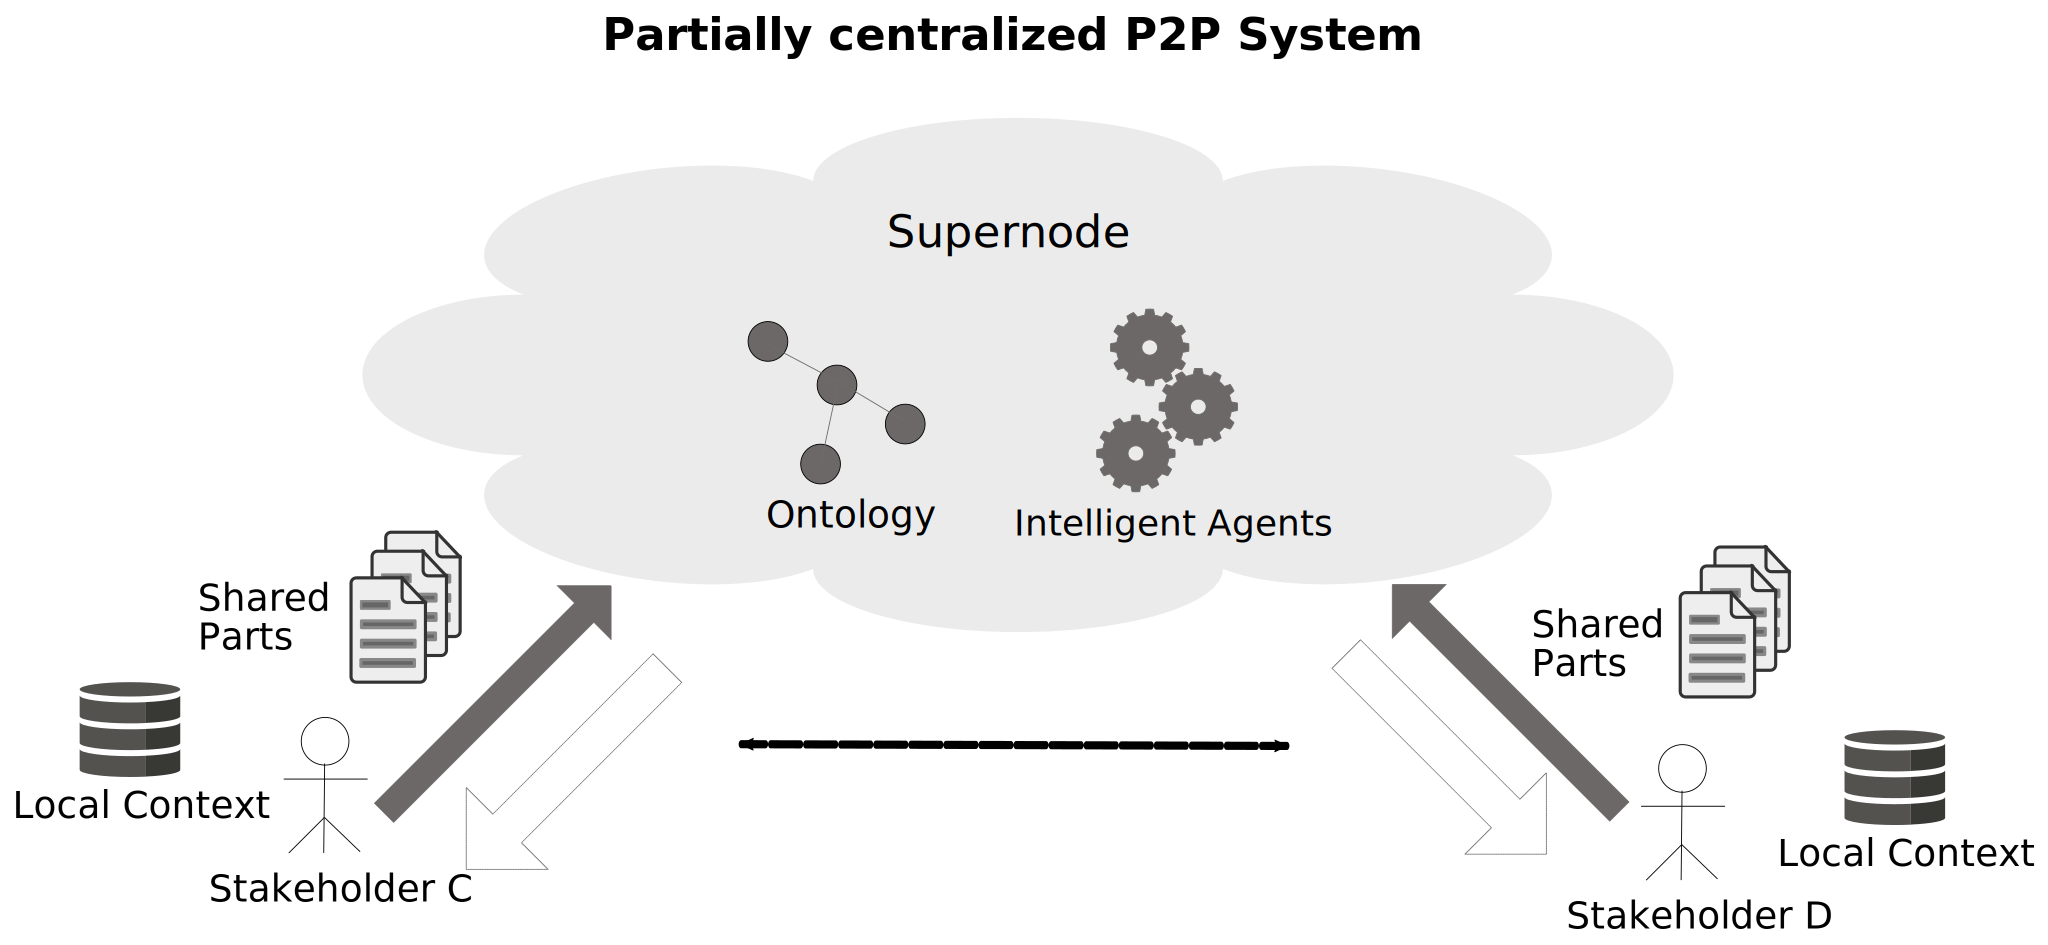
\includegraphics[width=0.9\columnwidth]{images/system_P2P_centralized.pdf}
	\caption{Collaborative system using a partially centralized \gls{P2P} architecture}
\label{fig:images_p2p_centralized}
\end{figure}


\subsection{Dealing with privacy concerns}
\label{subsec:p2p_partially_issuer_privacy}

One of the major issues with the above mentioned system architecture is, that the merchants, \gls{PSP}s and \gls{LSP}s have to hand over all of their relevant information to the issuer of a credit card for the analysis. \\
\ldots

% subsec p2p_partially_centralized_system

% section design_proposal (end)
